\documentclass[letterpaper]{article}
\usepackage{aaai}
\usepackage{times}
\usepackage{helvet}
\usepackage{courier}
\usepackage{subfig}
\usepackage{graphicx}
\frenchspacing
\pdfinfo{
/Title (PSMAGE: Procedural Starcraft MAp GEneration)
/Subject (AAAI Publications)
/Author (Alberto Uriarte, Jordan Santell)}
\setcounter{secnumdepth}{0}  
 \begin{document}
% The file aaai.sty is the style file for AAAI Press 
% proceedings, working notes, and technical reports.
%
\title{PSMAGE: Procedural Starcraft MAp GEneration}
\author{Alberto Uriarte \and Jordan Santell\\
Drexel University\\
Philadelphia\\
}
\maketitle
\begin{abstract}
\begin{quote}
Game designers can spend a lot of time tuning their maps to make it well balanced. This paper presents an algorithm for generating balanced maps for the popular real-time strategy (RTS) game StarCraft. We use Voronoi diagrams to randomly generate polygons as starting point. Then different properties are assigned to the polygons with some fitness functions in order to make consistent and balanced maps.
\end{quote}
\end{abstract}


\section{Introduction} % (fold)
\label{sec:introduction}
Procedural content generation (PCG) refers to the automatic or semi-automatic generation of game content. PCG comes in many flavors, as there are many types of game content that can be generated (such as levels, adventures, characters, weapons, planets, plants, histories, ...) and many ways in which it can be generated (many based on AI/CI methods such as constraint satisfaction, planning or evolutionary computation, ...). PCG can also be used in different ways in games, for example for offline content creation during game development, support tools for human designers or fully automatic online content creation based on player actions. Similarly, there are different motivations for using PCG, such as speeding up game development, saving human designer effort/cost, saving main memory or DVD storage, academic curiosity or the possibility of completely new types of games. What is clear, however, is that PCG is gaining increasing attention among both commercial game developers, indie developers and academic game researchers.
In this paper, we present an approach to generating maps to real-time strategy games. More specifically, we use an iterative process to generate maps for a tournament strategy games, where balance is key. Our algorithm automatically generate balanced maps for a specific strategy game: Starcraft.
% section introduction (end)


\section{Problem definition} % (fold)
\label{sec:problem_definition}


% section problem_definition (end)


\section{Related work} % (fold)
\label{sec:related_work}
This is not the first time where Starcraft maps are used as a testbed to do research. Luke Perkins developed the library BWTA to do terrain analysis on Starcraft maps \cite{Perkins10}. Z\'{e}pir researched on a Starcraft 2D map conversion into a Warcraft III 3D map \cite{Zepir}. And Togelius et al. also presented a methodology based on search for generating Starcraft maps \cite{Togelius10}.
% section related_work (end)


\section{Procedural map generation} % (fold)
\label{sec:procedural_map_generation}
The algorithm presented in this paper can be outlined as the following sequence of seven steps:
\begin{enumerate}
	\item Generate a random seed point
	\item Compute Voronoi diagram
	\item Add borders
	\item Compute region elevation
	\item Mirror map
	\item Parse output into a .chk file
	\item MPQ archive
\end{enumerate}
Each step shall now be described in detail. For illustrative purposes, the result of each step will be shown.

\subsection{1. Generate a random seed point}
First of all we must set the size of the map and the number of regions desired. Then we generate a random seed point for each region inside the map. The output of this step is shown in Figure \ref{fig:random-points}.

\begin{figure}[ht]
    \centering
    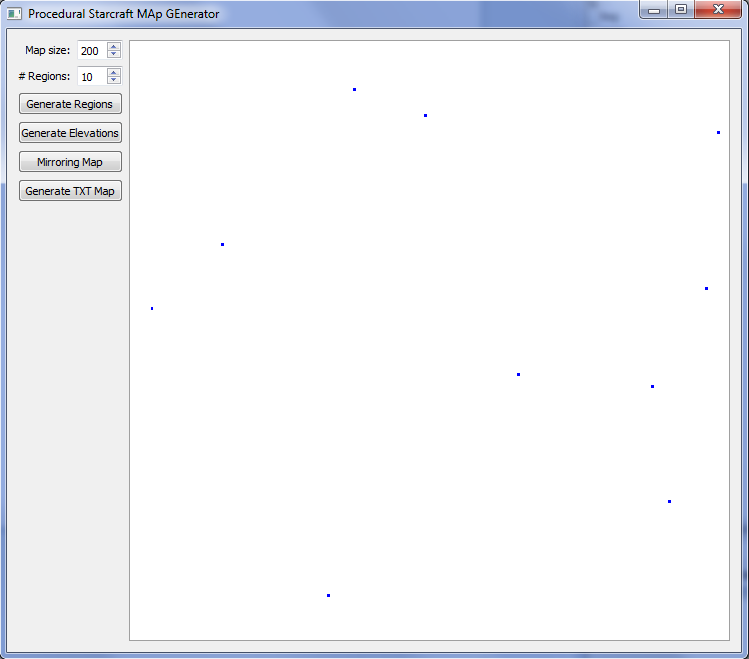
\includegraphics[width=8cm]{PCG01.png}
    \caption{Random points}
    \label{fig:random-points}
\end{figure}

\subsection{2. Compute Voronoi diagram}
The second step is to compute the Voronoi diagram from a set of points. This is accomplished using the fast Fortune's Algorithm \cite{Fortune}. This approach uses the idea of sweep line algorithms to design an efficient algorithm where its total time to process is O(\emph{n} log \emph{n}).

\subsection{3. Add borders}
The third step consists of generating the graph structure of regions. We represent region information as two related graphs: neighbors and edges.

The first graph has nodes for each adjacent region, which is useful for pathfinding algorithms. This graph is also known as Delaunay triangulation.

The second graph has nodes for each edge of the region. But the problem of Fortune's Algorithm is that it doesn't compute border map edges. To solve this we followed this steps:
\begin{enumerate}
	\item Detect regions with two edges ending on the same border.
	\item Create a new edge to link those edges.
	\item Detect regions with edges ending on different borders.
	\item Given a edge ending in a border, detect if the edge is in \emph{left/up} or \emph{right/bottom} side of the seed point. And expand the border in the right direction until find the second edge ending in a border.
\end{enumerate}
Now we are able to draw the polygon of each region as we shown in Figure \ref{fig:voronoi-diagram}.

\begin{figure}[ht]
    \centering
    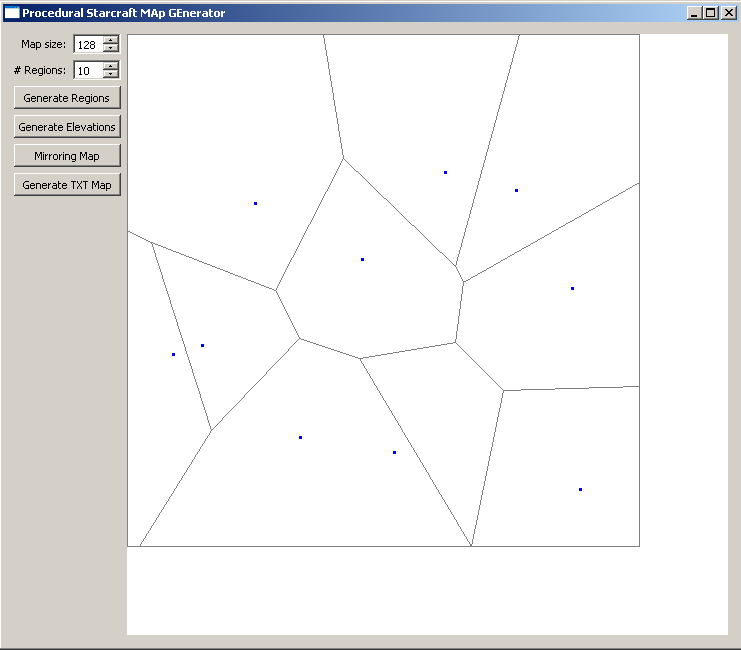
\includegraphics[width=8cm]{PCG02.png}
    \caption{Voronoi diagram}
    \label{fig:voronoi-diagram}
\end{figure}

\subsection{4. Compute region elevation}
In this step we decide the elevation of each region. Set the \% of hills regions (50 in our examples) and select randomly this regions. In this step we must ensure a path between the most left-up region to the most right-bottom region. This is because the most left-up region contains a starting point (location where a player start the game) and after the mirroring step each 1/4 parts of the map are connected through the initial most right-bottom region.

The fitness function to ensure this, it is an implementation of A* where the initial node is the most left-up region and the goal node is the most right-bottom region. We can use the neighbors graph described on step 3. If no path is found then we generate again the elevation info. Elevation information is shown in Figure \ref{fig:elevations}.

\begin{figure}[ht]
    \centering
    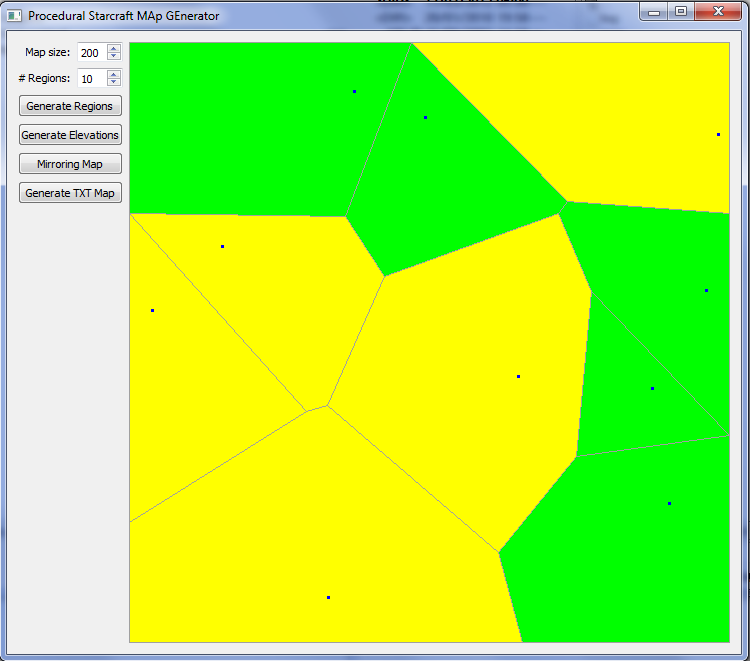
\includegraphics[width=8cm]{PCG03.png}
    \caption{Elevations}
    \label{fig:elevations}
\end{figure}

\subsection{5. Mirror map}
In order to get a balanced map like those used in Starcraft competitions, we perform a mirror transform over axis $x$ and axis $y$. First we duplicate all regions subtracting to each $x$ value of duplicated edges the double size of the width map size. As a result we have a map of size $2(mapWidth) \times (mapHeight)$. Then we duplicate again all regions subtracting to each $y$ value of duplicated edges the double size of the height map size. As a result, we have a balanced map of size $2(mapWidth)  \times 2(mapHeight)$ as shown in Figure \ref{fig:mirrored-map}.

\begin{figure}[ht]
    \centering
    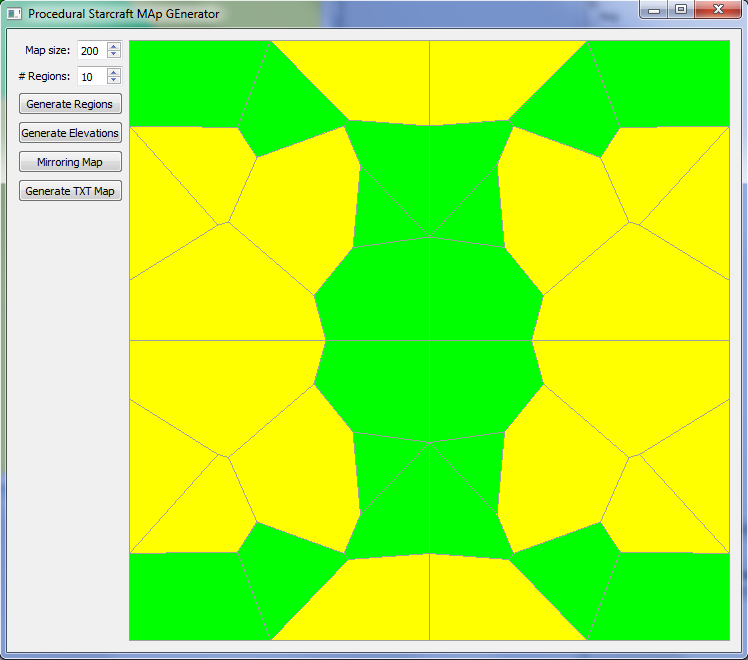
\includegraphics[width=8cm]{PCG04.png}
    \caption{Mirrored map}
    \label{fig:mirrored-map}
\end{figure}

\subsection{6. Parse output into a .chk file}
After mirroring our map, we generate a simple text output consisting of numbers assembled in a matrix format, where each number represents one tile, such that the output will have $(mapWidth) \times (mapHeight)$ numbers/tiles. The current values for output are 0 (water), 1 (low ground), and 2 (high ground).

Blizzard Entertainment uses their own archiving format for many of their games' files, the MPQ format. Starcraft is no exception, with map files (.scm, .scx) storing the map data in a CHK format, along with any other media used in that map, inside a MPQ archive. Using WinMPQ, we can extract the CHK file from the archive, which is a binary file containing up to 39 key-value pairs, where each section specifies information about the map, such as version information, terrain, custom options for units, upgrades and buildings and more. Each key contains 4 bytes of the section type, followed by a single 4 byte long (little-endian) indicating the length in bytes of the corresponding value immediately following the long \cite{Olbrantz}.

Example of CHK key-value in hexadecimal
\begin{verbatim}
43 4F 4C 52 08 00 00 00
00 01 02 03 04 05 06 07
\end{verbatim}

The first four bytes (43 4F 4C 52) represent the name of the section "COLR", followed by a 4 byte long (08 00 00 00), indicating the value for the section "COLR" will be 8 bytes long. For this section, each of the 8 bytes represents one of the eight players on the map, and their value can range from 0 to 15, indicating their color. In this example, player 1 is color 0 (red), player 2 is color 1 (blue), and so forth.

Each section has its own meaning on how to interpret their value, and can contain any combination of bytes, ints (2 bytes), longs (4 bytes) or chars (2 bytes). For example, the UNIx section contains unit settings for the level, which contains 4168 bytes of information for the 228 units in Brood War in a structured format of bytes and ints indicating the units' hit points, shield points, armor points, mineral and gas cost, current upgrade settings, and more.

Some of the sections' binary data was copied into our converter for use that were not related to terrain, such as the unit information/upgrades (PUPx, PTEx, UNIx, UPGx, TECx) and verification code (VCOD). Many more sections were filled with default data that are common in all non-custom maps, like version information and player information (TYPE, VER, IVE2, IOWN, OWNR, SIDE, PUNI, MASK, FORC) as well as the sections that are often used in heavily scripted Starcraft maps (STR, UPRP, UPUS, MRGN, TRIG, MBRF, SPRP, WAV, SWNM). We also set the sections related to doodads (objects that prevent movement on the map, like a statue) to their default values (DD2, THG2, MTXM).

Once a map file is set up with default settings, we bring in the text file output created by the Voronoi diagram previously and parse the map's dimensions (DIM), set a tileset (ERA=07, Twilight World) and set a tile value depending on the height of input. TILE is a matrix of 2 byte int tile values of $2 \times ((mapWidth)  \times (mapHeight))$ bytes, where each int represents what image should be painted on the ground at that coordinate. We use $37$ for low ground in our tileset and $67$ for high ground.

While Starcraft is based off of a grid, in the map editor, Staredit, users can change the terrain in isometric diamonds as in Figure /cite{iso-diamonds}, effectively affecting several tiles at once, easily creating "border" tiles, like cliffs where high and low terrain meet, randomizing the tile palette, and create a smooth, seamless environment.

\begin{figure}[ht]
    \centering
    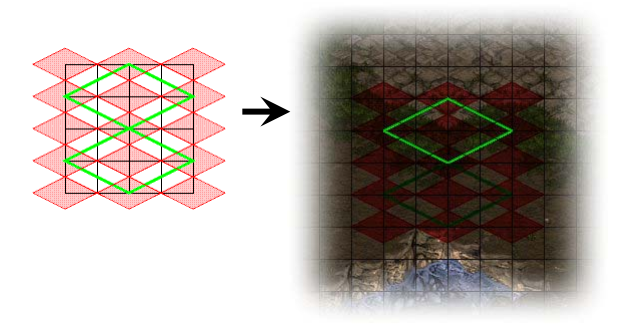
\includegraphics[width=8cm]{iso-diamonds.png}
    \caption{Isometric diamonds pattern}
    \label{fig:iso-diamonds}
\end{figure}

In the creation of a Starcraft to Warcraft 3 map conversion tool, Z\'{e}pir has done extensive documentation on the CHK's ISOM section, indicating each isometric diamond is described by 8 bytes, with 2 bytes describing each corner of a diamond \cite{Zepir}. While not yet implemented in our converter due to creating isometric data for every possible border combination, it is desirable.

\begin{figure*}[ht]
  \centering
  \subfloat[Tileset Desert Wrold]{
\includegraphics[width=0.33\textwidth]{desertworld.png}}
  ~ %add desired spacing between images, e. g. ~, \quad, \qquad etc. (or a blank line to force the subfig onto a new line)
  \subfloat[Tileset Space Platform]{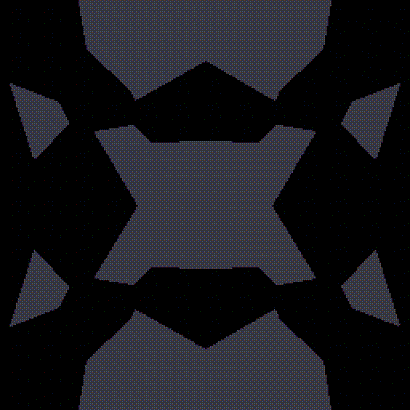
\includegraphics[width=0.33\textwidth]{spaceplatform.PNG}}
  ~ %add desired spacing between images, e. g. ~, \quad, \qquad etc. (or a blank line to force the subfig onto a new line)
  \subfloat[Tileset Twilight World]{
\includegraphics[width=0.33\textwidth]{twilight.PNG}}
  \caption{Starcraft generated map with different tilesets}
  \label{fig:final-maps}
\end{figure*}

\subsection{7. MPQ archive}
MPQ (MoPaQ) is an archive format developed by Blizzard Entertainment, purposed for storing data files, images, sounds, music and videos for their games. The name MoPaQ comes from the author of the format, Mike O'Brien (Mike O'brien PaCK). So far, MPQ archives have been used for the following games:
\begin{itemize}
	\item Diablo
	\item StarCraft
	\item Warcraft II (Battle.net Edition)
	\item Diablo II
	\item Warcraft III
	\item World of Warcraft
	\item Starcraft II
	\item Lord of Magic (by Sierra)
	\item Hellfire (Diablo datadisk by Sierra)
\end{itemize}

They designed this archive format with the following reguirements:
\begin{description}
	\item[Security] Blizzard didn't want people to access their files and thus hack their games. Archive format must have supported data encryption.
	\item[Fast access] It was necessary to access archived data as fast as possible, in realtime.
	\item[Compression] Blizzard decided to store sound files, including music, in the WAV format. Uncompressed size of these files is very large and archive must support a compression. Several compression methods are used to store data files within MPQ archives (PKWARE Data Compression Library, ZLIB, BZIP2, LZMA and SPARSE compression), together with Huffman and IMA ADPCM compression methods used for storing WAV files.
	\item[Expandability] Archive format must support later changes of the way how the files are stored in the archive. With new games released, the MPQ format is being extended. All the later changes are backward-compatible with older versions.
	\item[Multilanguage] Blizzard planned to release its games worldwide, in various language versions. The archive format must support storing multiple files with different languages.
\end{description}

Upon the export of the CHK file, we can put it back into an MPQ archive, or we can just rename the file extension to .scx and open the file in Staredit/Starcraft.

% section procedural_map_generation (end)


\section{Implementation} % (fold)
\label{sec:implementation}
This algorithm has been implemented in C++ for the map generation and Ruby for the conversion into a Starcraft map format. Additionally, PSMAGE uses the Qt framework to draw the results of each step. Additionally, WinMPQ was used to pull out CHK files from the MPQ archives, and AXE 3 to view and debug the binary CHK files.
% section implementation (end)


\section{Results} % (fold)
\label{sec:results}
Figure \ref{fig:final-maps} depicts maps resulting from our algorithm with different tilesets.

Our PCG algorithm classify as follows:
\begin{description}
	\item[Offline] It takes place during game design.
	\item[Necessary] The content generated is necessary to play a tournament game.
	\item[Control vector] We defined some features (map size, number of regions, \% hills) which a game designer can decide.
	\item[Stochastic] Given the same features the output is unpredictable.
	\item[Constructive and Generate \& Test] Some steps are purely designed to give a valid output, but some others steps must satisfy a fitness function.
\end{description}

% section results (end)


\section{Conclusion} % (fold)
\label{sec:conclusion}
In this paper, we used an iterative algorithm with a map graph structure. We defined some constraints and some fitness functions measuring map qualities. We have also develop a basic matrix map converter to Starcraft map format. We believe that our maps are comparable with those made by humans for a tournament game propose, and can be used for completely automated map generation and to assist human map designers.

Future work will deal with some points that we didn't have time to test:
\begin{itemize}
	\item A better random seed points distribution (maybe a poison distribution). Since the default random numbers are more "clumpy" than what people expect.
	\item Use Lloyd's relaxation to smooth regions.
	\item Experiment with other mirroring techniques.
	\item Fitness function to add ramps on edges.
	\item Add another step to adding some tile noise and static objects.
	\item Implement correct isometric mapping to create borders and maps that visually look like they were created in Staredit that are playable.
\end{itemize}

% section conclusion (end)


%%%%%%%%%%
% References and End of Paper
\bibliography{psmage}
\bibliographystyle{aaai}
\end{document}